The given equation can be expressed as a parabola with parameters

\begin{align}
\vec{V} = \myvec{1 & 0 \\ 0 & 0},\vec{u}=\myvec{0 \\ \frac{-1}{2}},f = -3
\end{align}
Using eigenvalue decomposition,
\begin{align}
\vec{D} = \myvec{0 & 0\\0 & 1} ,\vec{P}=\myvec{0 & 1\\1 & 0}
\end{align}
and
\begin{align}
\myvec{\vec{u}^T + \eta\vec{p_1}^T \\ \vec{V}}\vec{c} &= \myvec{-f \\ \eta\vec{p_1}-\vec{u}} 
\\
\implies \myvec{0 & -1 \\ 1 & 0 \\ 0 & 0}\vec{c} &= \myvec{3 \\ 0 \\ 0} \\
\implies  \myvec{0 & -1 \\ 1 & 0}\vec{c} &= \myvec{3 \\ 0}
\\
\implies \vec{c} &= \myvec{0\\-3}
\end{align}
%
The zeros are at $\pm \sqrt{3}$, which can be verified in Fig. \ref{quadform/2/19/dex3}.	
\begin{figure}[!ht]
\centering
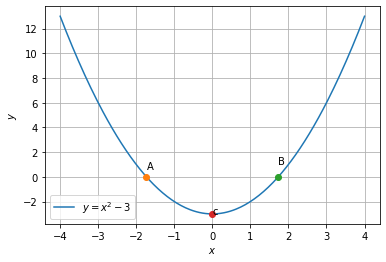
\includegraphics[width=\columnwidth]{solutions/su2021/2/19/d/download (3).png}
\caption{$y=x^2-3$}
\label{quadform/2/19/dex3}	
\end{figure}
